\documentclass[11pt,oneside,openany,itemph,a4paper,chapter]{oblivoir}

\usepackage[table,xcdraw]{xcolor}
\usepackage{pdfpages}
\usepackage{float}
\usepackage{graphicx}
\usepackage{fancyvrb}
\usepackage{fvextra}
\usepackage{siunitx}
\usepackage{titlesec}
\usepackage{titling}
\usepackage{fontspec}
\usepackage{makeidx}
\usepackage{array}
\usepackage{tabularx}
\newcolumntype{P}[1]{>{\raggedright\arraybackslash}p{\dimexpr#1-2\tabcolsep-1.5\arrayrulewidth}}
\newcolumntype{K}[1]{>{\raggedright\arraybackslash}p{\dimexpr#1-2\tabcolsep-1.25\arrayrulewidth}}

\usepackage{booktabs}
\usepackage{makecell}
\setcellgapes{6pt}
\makegapedcells

\usepackage{subfig}
\renewcommand*{\thesubfigure}{\arabic{subfigure}}
\usepackage{geometry}

\pagestyle{hangul}

\usepackage{fapapersize}
% width, height, left, right, upper, lower
% \usefapapersize{210mm,290mm,30mm,*,20mm,25mm}

\disablekoreanfonts
\setmainfont[BoldFont={KoPubWorldDotumPM}]{KoPubWorldBatangPL}
\setmonofont{D2Coding}

\newfontfamily\headingfont[]{KoPubWorldDotumPM}
\renewcommand{\maketitlehooka}{\headingfont}

\SetHangulspace{1.6}{1.2}

\newenvironment{tablekeyvalue}[2]
{\bgroup
\table[H] \tabularx{\linewidth}{|
>{\setlength{\baselineskip}{1.2\baselineskip}}P{#1\linewidth}|
>{\setlength{\baselineskip}{1.2\baselineskip}}P{#2\linewidth}|}
\hline}
{\endtabularx \endtable \egroup}

\title{자체 평가 결과 보고서\\3차원 기하 모델 프로세싱 프레임워크 개발}
\author{KAIST 전산학부 기하컴퓨팅연구실}
\date{2020년 12월 9일}

\makeindex

\begin{document}

\frontmatter
\maketitle
\newpage
\tableofcontents
% \listoffigures
% \listoftables

\mainmatter

\chapter{평가 개요}

\section{요약}
\begin{tablekeyvalue}{0.2}{0.8}
평가 대상 & 3차원 기하 모델 프로세싱 프레임워크 v2.0\\ \hline
평가 일시 & 2020년 12월 9일 \\ \hline
평가 버전 & 평가 시점 현재, GitHub을 활용하여 관리 및 공개하고 있는 최신 소스 코드 \\ \hline
평가 방법 & GitHub을 활용하여 관리 및 공개하고 있는 자동 평가 스크립트의 실행에 의한 자동 시험 \\ \hline
평가 결과 & 정량적 목표 항목 100\% 달성 \\ \hline
\end{tablekeyvalue}

\section{정량적 목표 항목별 결과 요약}

\bgroup
\begin{table}[H]
\begin{tabularx}{\linewidth}{
|>{\setlength{\baselineskip}{1.2\baselineskip}}K{0.4\linewidth}
|K{0.15\linewidth}|K{0.15\linewidth}|K{0.3\linewidth}|}
\hline
평가 항목 & 목표치 & 달성 & 관련 테스트 \\ \hline
지원 3차원 모델 형식 개수 & 4개 & 4개 & 평가 \#1, \pageref{test1}~페이지 \\ \hline
단일 3차원 모델 크기 & 100 MB & 144 MB & 평가 \#1, \pageref{test1}~페이지 \\ \hline
준 실시간 모니터링 통계 자료 입도 & 15분 & 15분 & 평가 \#2, \pageref{test2}~페이지 \\ \hline
업무 처리용 화면 개수 & 27개 & 27개 & 평가 \#3, \pageref{test3}~페이지 \\ \hline
서비스 초기 구축 시간 & 10분 & 2분 21초 & 평가 \#3, \pageref{test3}~페이지 \\ \hline
\end{tabularx}
\end{table}
\egroup

\section{평가 대상 버전}
평가 시점 현재 GitHub을 활용하여 관리 및 공개하고 있는 자동 테스트 스크립트 저장소 main branch의 최신 소스 코드를 평가 직전 clone하였다. 평가 시점에 받은 실제 Git 커밋은 아래 표와 같다. 이 저장소의 자동 테스트 스크립트는 다시 테스트 실행 시점 최신 소스 코드를 clone한다.

\begin{tablekeyvalue}{0.3}{0.7}
kaist-gclab/delta-test-report & eda13dbad0260b34384eaffd036074fc7a5a948e \\ \hline
\end{tablekeyvalue}

\section{평가 방법}
자동적으로 정량적 목표 항목 평가를 수행하는 스크립트를 작성하였으며, 스크립트의 내용을 모두 GitHub 저장소 kaist-gclab/delta-test-report에 공개하였다. 본 자체 평가 결과 보고서의 결과 수치는 사람의 개입을 배제하고 공개되어 있는 스크립트의 실행을 통한 자동 시험에 의하여 얻은 것이다. 누구든지 스크립트를 다운로드 및 실행하여, 동등한 결과가 출력되는 것을 확인할 수 있다. 특히 전체 시스템을 이루는 핵심 구성 요소인 데이터베이스 서버, 애플리케이션 서버, 오브젝트 저장소의 실행 환경 구성과 설치가 Docker로 이루어지도록 하여 테스트의 재현성을 크게 높였다. 단, 평가 \#1은 100 MB 이상의 3차원 모델을 소스 코드 저장소에 함께 보관하는 것이 곤란한 점, 렌더링 결과는 이미지 형태로 나타나므로 자동화 테스트를 통한 적부 판정이 어려워 사람의 눈으로 확인해야 하는 점을 고려하여 별도로 수행하는 한편, 테스트 수행 상세 방법을 명시하였다.

정량적 목표 중 수행 시간처럼 실제 테스트가 수행되는 시스템의 성능에 영향을 받을 수 있는 항목의 달성 여부는 평가 환경에 따라 달라질 수 있다. 본 보고서 작성에 이용된 시스템의 상세 사양 등 평가 환경은 다음 장에 서술하였으며, 본 보고서의 평가 범위는 보고서에 명시된 평가 환경과 평가 내용으로 한정한다.

\section{평가 환경}
\subsection{하드웨어}
\begin{tablekeyvalue}{0.2}{0.8}
CPU & Intel(R) Core(TM) i7-6800K CPU @ 3.40GHz \\ \hline
RAM & 64 GB \\ \hline
SSD & 240 GB \\ \hline
HDD & 4 TB \\ \hline
네트워크 & 100 Mbps \\ \hline
온도 & 17 \si{\celsius} (서버실 냉방기 설정 온도) \\ \hline
\end{tablekeyvalue}
\subsection{소프트웨어}
\begin{tablekeyvalue}{0.2}{0.8}
운영체제 & Ubuntu 20.04.1 LTS \\ \hline
Docker & 19.03.13, build 4484c46d9d \\ \hline
셸 & GNU bash, version 5.0.17(1)-release (x86\_64-pc-linux-gnu) \\ \hline
Node.js & v14.15.1 \\ \hline
npm & 6.14.9 \\ \hline
\end{tablekeyvalue}

\chapter{평가 내용}


\section{평가 \#1\label{test1} 3차원 모델 렌더링 테스트}

자체 평가 결과의 재현성과 신뢰성을 제고하기 위하여, 테스트에 이용한 대용량 3차원 모델은 공개적으로 구할 수 있는 3차원 모델을 이용하였다. 테스트에 이용한 3차원 모델은 `보물 제1142호 경주 죽동리 청동기 일괄'이며, 문화재청 국가문화유산포털에서 취득하였다. 이 3차원 모델은 사람이 모델링한 것이 아닌, 문화재를 3D 스캐너로 스캔하는 방법으로 작성되었기 때문에 스캔 과정에서 발생하는 잡음 등이 포함되어 구조가 매우 복잡하며, 문화재를 보존하기 위한 목적상 고해상도로 스캔되었다.
\begin{quote}
    문화재청에서 2018년 작성하여 공공누리 제1유형으로 개방한 `보물 제1142호 경주 죽동리 청동기 일괄'을 이용하였으며, 해당 저작물은 문화재청, 공공데이터포털에서 무료로 다운받을 수 있습니다.
\end{quote}

\subsection{평가 항목}
\subsubsection{지원 3차원 모델 형식 개수}
3차원 모델 형식은 매우 다양하며, 형식에 따라 장점과 단점이 모두 있어, 3차원 모델을 다루는 분야에서는 특정한 3차원 모델 형식으로 통일하지 않고 상황에 맞는 3차원 모델 형식을 사용한다. 본 시스템은 개인이나 기업, 연구소 등에서 다루는 수많은 3차원 모델 형식을 하나의 저장소에 통합하여 관리하는 상황을 고려해야 하므로, 다양한 3차원 모델 형식을 지원하는 것이 필수적이다.

\subsubsection{단일 3차원 모델 크기}
3차원 인터랙티브 컴퓨터 그래픽스, 3D 프린팅과 같은 응용 분야에서 모델이 적절하게 최적화되어 있는 경우, 단일 3차원 모델로서 100MB는 일반적인 범위를 뛰어넘는 충분한 용량이다. 평가에는 문화재청에서 공공누리 제1유형으로 공개하여 문재재청 및 공공데이터포털에서 무료로 다운로드할 수 있는 대용량 3차원 모델을 이용하였다.

\subsection{평가 절차}
\begin{enumerate}
    \item GitHub에서 delta-renderer 저장소를 다운로드한다.
    \item Docker Hub에서 delta-renderer-base를 다운로드한다.
    \item Docker로 delta-renderer-base를 실행하고, delta-renderer/renderer/build.sh을 이용하여 렌더러를 빌드한다. 이 과정은 서버와 별도로, 렌더러만 빌드하여 렌더러의 지원 형식 개수와 지원하는 3차원 모델 크기를 측정하는 절차다.
    \item delta-renderer/renderer/run.sh을 이용하여 렌더링 결과 이미지를 생성한다.
    \item 렌더링 결과 이미지가 예상한 이미지와 일치하는지 확인한다.
\end{enumerate}

\subsection{평가 모델}
\begin{enumerate}
    \item 보물 제1142호 경주 죽동리 청동기 일괄, model/x.stl-ascii
    \item 보물 제1142호 경주 죽동리 청동기 일괄, model/x.stl-binary
    \item 유타 주전자, model/obj
    \item 유타 주전자, model/delta
\end{enumerate}

\subsection{평가 결과}

`보물 제1142호 경주 죽동리 청동기 일괄'과 유타 주전자 모두 예상한 결과 이미지와 동일한 이미지가 렌더링되었다. 렌더링은 각도를 일정한 간격으로 증가시키면서 32번 수행되었으며, 아래 이미지는 32장의 이미지를 하나로 병합한 것이다. `보물 제1142호 경주 죽동리 청동기 일괄, model/x.stl-ascii' 모델의 크기는 144 MB이며, 정량적 목표 100 MB를 넘어선다.

\begin{figure}[h]
\centering
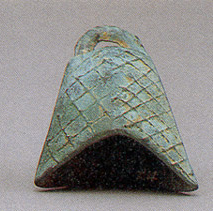
\includegraphics[width=0.3\textwidth]{real.png}
\caption{보물 제1142호 경주 죽동리 청동기 일괄 실제 사진}
\end{figure}

\begin{figure}[h]
\centering
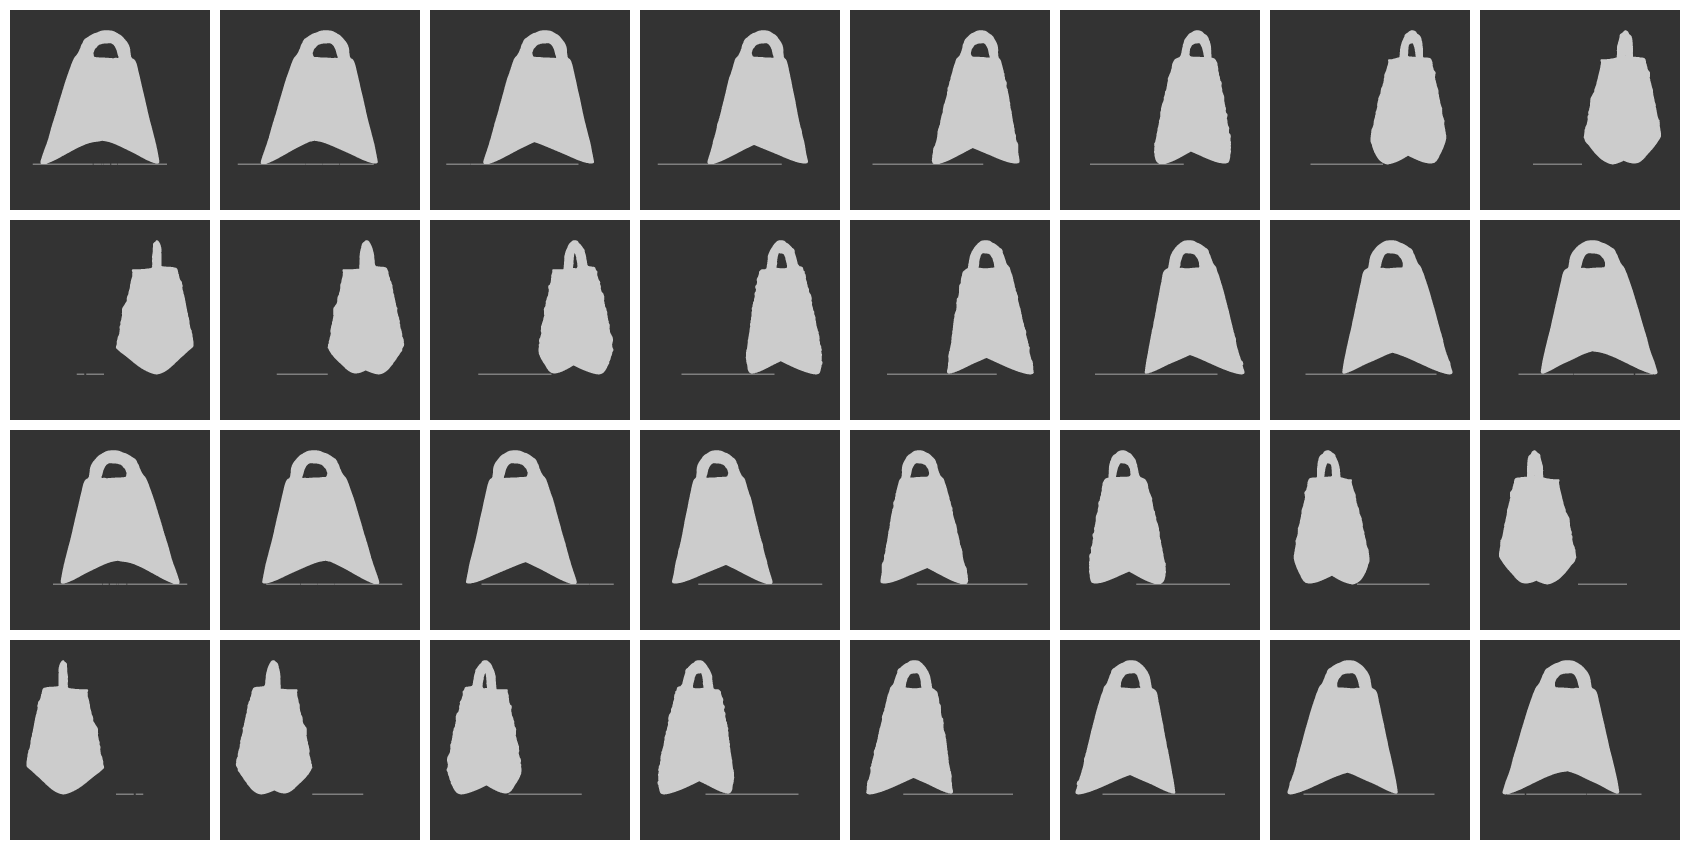
\includegraphics[width=\textwidth]{rendered.png}
\caption{보물 제1142호 경주 죽동리 청동기 일괄 렌더링 결과}
\end{figure}

\begin{figure}[h]
\centering
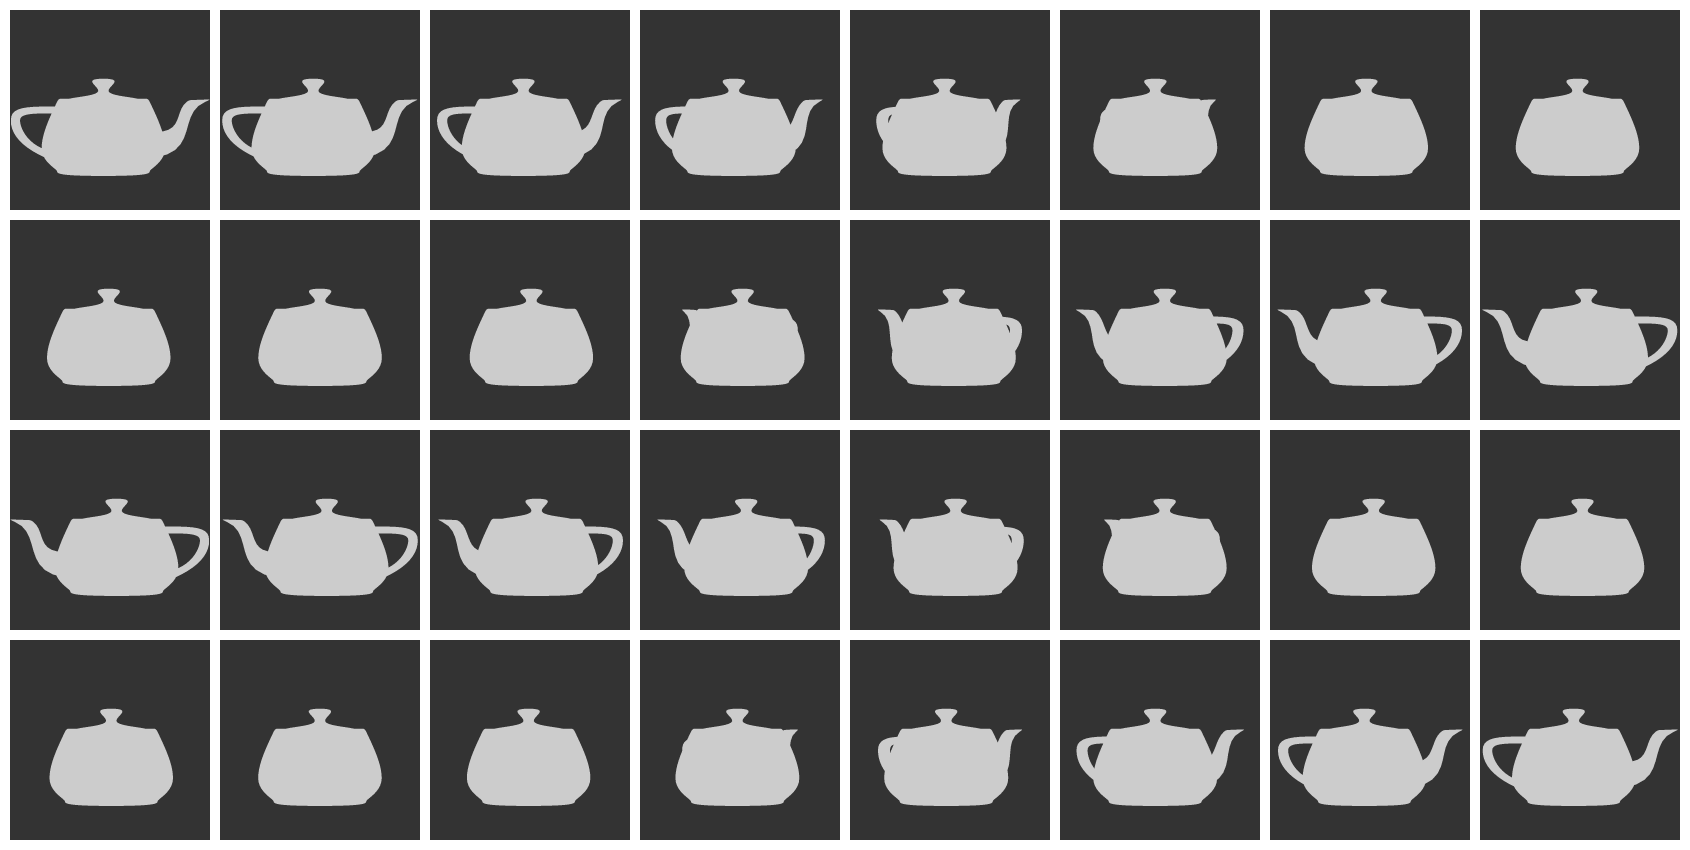
\includegraphics[width=\textwidth]{teapot.png}
\caption{유타 주전자 렌더링 결과}
\end{figure}

\begin{tablekeyvalue}{0.3}{0.7}
지원 3차원 모델 형식 개수 & 전체 4종의 3차원 모델 형식 model/x.stl-ascii, model/x.stl-binary, model/obj, model/delta의 렌더링 결과, 예상한 결과 이미지와 동일한 이미지가 출력되었다. \\ \hline
단일 3차원 모델 크기 & 144 MB의 대용량 3차원 모델을 렌더링하였으며, 예상한 결과 이미지와 동일한 이미지가 렌더링되었다. \\ \hline
\end{tablekeyvalue}

\section{평가 \#2\label{test2} 모니터링 기능 테스트}
\subsection{평가 항목}
\subsubsection{준 실시간 모니터링 통계 자료 입도}
시스템 상태 감시를 위한 통계 자료를 수집할 때 너무 짧은 간격으로 수집하면 시스템 성능뿐만 아니라 데이터의 양이 매우 많아지므로, 일반적으로 분 단위, 시간 단위, 일 단위 등으로 집합적인 통계 자료를 수집한다. 합리적인 수준의 지연을 사용하면서 동시에 적당한 통계 자료 입도(granularity, 세분성)를 제공하는 것이 본 평가 항목의 목적이다.

\subsection{평가 절차}
3차원 기하 모델 프로세싱 프레임워크는 대량의 로그를 처리할 목적으로 InfluxDB를 사용하고 있으며, InfluxDB는 자체적으로 대량의 시계열 데이터가 들어왔을 때 시계열 데이터의 보존 기간을 설정하여 데이터를 제거하거나 연속된 데이터를 그룹화하여 집합적으로 다룰 수 있는 기능이 있다. 3차원 기하 모델 프로세싱 프레임워크는 로그 데이터의 그룹화와 보존 기간 설정을 전적으로 InfluxDB에 의존하므로, 모니터링 통계 자료 입도 검증에 있어서는 프레임워크의 동작을 테스트(test)하는 것이 아닌, 정확한 방법으로 InfluxDB와 연동되어 있는지를 소스 코드에서 직접 검사(inspect)하는 것이 바람직하다.
\begin{enumerate}
    \item 소스 코드에서 InfluxDB와 연동하는 부분을 확인한다.
    \item 그룹화 설정이 정확히 15분으로 설정되어 있는지 검사한다.
\end{enumerate}

\subsubsection{소스 코드 검사}
본 시스템은 InfluxData가 공식적으로 제공하는 InfluxDB.Client를 이용하여 InfluxDB와 연결하고 있으며, continuous query 기능을 이용하여 다운 샘플링을 수행하고 있다. 예를 들어, 본 프레임워크는 오브젝트 저장소의 전체 크기를 수집하고 있으며, 실제 질의문의 내용은 아래와 같다. Continuous query에서는 그룹화 설정을 GROUP BY time()로 나타내며, 15m는 15분을 의미한다.

\begin{verbatim}
CREATE CONTINUOUS QUERY "downsample-object-storage" ON "delta"
BEGIN
    SELECT mean("total-size")
    INTO "average-object-storage"
    FROM "object-storage"
    GROUP BY time(15m)
END
\end{verbatim}

\subsection{평가 결과}
\begin{tablekeyvalue}{0.3}{0.7}
준 실시간 모니터링 통계 자료 입도 & 입도가 15분으로 설정되어 있어, 전체 로그가 아닌 15분 평균 데이터가 처리되고 있음을 소스 코드 검사로 확인하였다. \\ \hline
\end{tablekeyvalue}

\section{평가 \#3\label{test3} 서비스 자동 구축 테스트}
\subsection{평가 항목}
\subsubsection{업무 처리용 화면 개수}
정량적인 평가 항목만 만족하는 연구 개발 사업이 아닌, 종료 후에도 지속적으로 사용, 발전될 수 있는 소프트웨어가 되려면 소스 코드의 일부분 공개가 아닌 실제 사용 가능한 인터페이스가 있는 완전한 소프트웨어를 공개해야 한다. 인터페이스 구현을 정량적으로 측정하기 위하여 화면(기능) 개수를 평가 항목으로 제안하였으며, 화면 27개는 인접 분야의 이미 상용화된 유사 소프트웨어를 기준으로 하였다.

\subsubsection{서비스 초기 구축 시간}
서비스 초기 구축 시간의 고성능 여부를 결정하는 절대적인 기준은 없으나, 대표적인 클라우드 서비스 제공자 중 하나인 Amazon의 공식 사용자 튜토리얼에서 Amazon EC2 서비스를 설치하는 데 걸리는 시간은 10분으로 소개되어 있다. 운영 체제 설치 등은 제외한, 시스템 하드웨어와 기본 소프트웨어가 준비되어 있는 상태에서 설치 완료까지 걸리는 시간으로 평가한다.

\subsection{평가 절차}
\begin{enumerate}
    \item GitHub에서 delta-test-report 저장소를 다운로드한다.
    \item 서버에 이미 다운로드된 이미지가 있어 서비스 구축 시간이 단축되는 등 엄정한 평가에 영향을 주는 요소를 제거하기 위하여, docker rmi \$(docker images -q) 및 sudo rm -rf ./temp 명령을 수행한다.
    \item ./run.sh 스크립트를 실행한다. 해당 스크립트는 Ubuntu 및 macOS 최신 안정 버전에서 정상 동작이 확인되었다.
    \item 스크립트 종료 이후, log.txt에 포함된 타임스탬프를 이용하여 구축 소요 시간을 확인한다.
    \item 스크립트 종료 이후, output 디렉터리에 포함된 이미지를 확인하여 27개의 업무 처리용 화면 스크린샷이 보관된 것을 확인한다.
\end{enumerate}

\subsection{평가 결과}
자동 구축 스크립트에 의한 시스템 구축이 성공적으로 이루어졌으며, 구축 완료 이후 웹 브라우저에서 즉시 접근할 수 있었다. 자동 구축은 2020년 12월 9일 수요일 18:17:09에 시작되어, 2020년 12월 9일 수요일 18:19:30에 종료되었다. 두 타임스탬프의 차이는 2분 21초이며, 목표치인 10분보다 짧은 결과이다. 서비스 구축 소요 시간 계산에는 Ubuntu 운영체제 설치 및 이미지 다운로드, PostgreSQL 다운로드 등 본 3차원 기하 모델 프로세싱 프레임워크와 직접적인 관계가 없는 소프트웨어를 준비하는 시간을 제외하였다. 그러나 직접적으로 3차원 기하 모델 프로세싱 프레임워크와 관계가 있는, 프레임워크 구성 요소 소스 코드 다운로드 시간, 프레임워크 구성 요소 Docker 빌드 시간, 프레임워크 구성 요소 첫 실행 시간 등은 모두 서비스 구축 소요 시간에 합산하였다.

자동 구축 완료에 이어 곧바로 Chrome 웹 브라우저 자동화 도구인 Puppeteer를 이용하여 27개의 업무 처리용 화면을 방문하고 스크린샷을 보관하도록 한 결과, 모든 화면 방문과 스크린샷 저장이 성공적으로 완료되었으며 본 연구 개발 사업 2차 연도 연차 보고서 및 도움말에 설명된 27개의 기능이 확인되었다.

\begin{tablekeyvalue}{0.3}{0.7}
    업무 처리용 화면 개수 & 27개의 업무 처리용 화면이 성공적으로 표시된 것을 확인하였다. \\ \hline
    서비스 초기 구축 시간 & 3차원 기하 모델 프로세싱 프레임워크가 설치되어 있지 않은 상태에서, 다운로드 및 설치, 서비스 시작까지 소요된 시간은 2분 21초였다. \\ \hline
\end{tablekeyvalue}

\newgeometry{left=0.5cm,top=0.5cm,right=0.5cm,bottom=0.5cm}
\begin{figure}[h]
\centering
\begin{tabular}{cccc}
    \subfloat[로그인]{\includegraphics[width=3.5cm]{../../output/01.png}} &
    \subfloat[시작]{\includegraphics[width=3.5cm]{../../output/02.png}} &
    \subfloat[도움말]{\includegraphics[width=3.5cm]{../../output/03.png}} &
    \subfloat[사용자 설정]{\includegraphics[width=3.5cm]{../../output/04.png}} \\
    \subfloat[시스템 설정]{\includegraphics[width=3.5cm]{../../output/05.png}} &
    \subfloat[에셋 추가]{\includegraphics[width=3.5cm]{../../output/06.png}} &
    \subfloat[에셋 목록]{\includegraphics[width=3.5cm]{../../output/07.png}} &
    \subfloat[에셋 상세 조회]{\includegraphics[width=3.5cm]{../../output/08.png}} \\
    \subfloat[에셋 뷰어]{\includegraphics[width=3.5cm]{../../output/09.png}} &
    \subfloat[에셋 유형 추가]{\includegraphics[width=3.5cm]{../../output/10.png}} &
    \subfloat[에셋 유형 목록]{\includegraphics[width=3.5cm]{../../output/11.png}} &
    \subfloat[에셋 유형 상세 조회]{\includegraphics[width=3.5cm]{../../output/12.png}} \\
    \subfloat[뷰어 목록]{\includegraphics[width=3.5cm]{../../output/13.png}} &
    \subfloat[작업 추가]{\includegraphics[width=3.5cm]{../../output/14.png}} &
    \subfloat[작업 목록]{\includegraphics[width=3.5cm]{../../output/15.png}} &
    \subfloat[작업 상세 조회]{\includegraphics[width=3.5cm]{../../output/16.png}} \\
    \subfloat[작업 유형 목록]{\includegraphics[width=3.5cm]{../../output/17.png}} &
    \subfloat[작업 유형 상세 조회]{\includegraphics[width=3.5cm]{../../output/18.png}} &
    \subfloat[처리기 노드 목록]{\includegraphics[width=3.5cm]{../../output/19.png}} &
    \subfloat[처리기 노드 상세 조회]{\includegraphics[width=3.5cm]{../../output/20.png}} \\
    \subfloat[암호화 키 추가]{\includegraphics[width=3.5cm]{../../output/21.png}} &
    \subfloat[암호화 키 목록]{\includegraphics[width=3.5cm]{../../output/22.png}} &
    \subfloat[암호화 키 상세 조회]{\includegraphics[width=3.5cm]{../../output/23.png}} &
    \subfloat[모니터링 대시보드]{\includegraphics[width=3.5cm]{../../output/24.png}} \\
    \subfloat[오브젝트 저장소 \newline 모니터]{\includegraphics[width=3.5cm]{../../output/25.png}} &
    \subfloat[처리기 노드 모니터]{\includegraphics[width=3.5cm]{../../output/26.png}} &
    \subfloat[작업 모니터링]{\includegraphics[width=3.5cm]{../../output/27.png}}
\end{tabular}
\end{figure}
\restoregeometry

\chapter{상세 테스트 로그 원본}

\section{테스트 \#3 서비스 자동 구축 테스트}
\begin{Verbatim}[fontsize=\tiny, breaklines=true, breakanywhere=true]
이전 테스트에서 제거되지 않았을지도 모르는 잔여 파일 및 Docker 컨테이너를 모두 제거합니다.
서버 구축 시작 시각입니다. 지금부터 서버 구축 시간을 측정합니다.
2020. 12. 09. (수) 18:17:09 KST
3차원 기하 모델 프로세싱 프레임워크를 다운로드합니다. 이 다운로드 단계는 서버 구축 시간에 포함합니다.
3차원 기하 모델 프로세싱 프레임워크를 빌드합니다.
데이터베이스 서버 초기화 작업이 완료될 수 있도록 60 초 더 기다립니다.
서버 구축 완료 시각입니다.
2020. 12. 09. (수) 18:19:30 KST
자동 테스트를 시작합니다.
2020-12-09 18:19:33.431 screens	INFO	screens
2020-12-09 18:19:33.597 screens	INFO	웹 서버 주소 http://localhost:28080/
2020-12-09 18:19:33.960 screens	INFO	로그인 페이지로 이동 완료
2020-12-09 18:19:34.061 screens	INFO	암호 입력 완료
2020-12-09 18:19:34.164 screens	INFO	스크린샷 output/01.png 저장 완료
2020-12-09 18:19:34.190 screens	INFO	로그인 버튼 클릭 완료
2020-12-09 18:19:34.857 screens	INFO	로그인 성공
2020-12-09 18:19:34.862 screens	INFO	시작 페이지 메뉴 항목 발견
2020-12-09 18:19:34.877 screens	INFO	시작 페이지로 이동 시작
2020-12-09 18:19:34.879 screens	INFO	시작 페이지로 이동 성공
2020-12-09 18:19:34.956 screens	INFO	스크린샷 output/02.png 저장 완료
2020-12-09 18:19:34.962 screens	INFO	도움말 페이지 메뉴 항목 발견
2020-12-09 18:19:34.975 screens	INFO	도움말 페이지로 이동 시작
2020-12-09 18:19:34.977 screens	INFO	도움말 페이지로 이동 성공
2020-12-09 18:19:35.035 screens	INFO	스크린샷 output/03.png 저장 완료
2020-12-09 18:19:35.041 screens	INFO	사용자 설정 페이지 메뉴 항목 발견
2020-12-09 18:19:35.053 screens	INFO	사용자 설정 페이지로 이동 시작
2020-12-09 18:19:35.055 screens	INFO	사용자 설정 페이지로 이동 성공
2020-12-09 18:19:35.122 screens	INFO	스크린샷 output/04.png 저장 완료
2020-12-09 18:19:35.127 screens	INFO	시스템 설정 페이지 메뉴 항목 발견
2020-12-09 18:19:35.141 screens	INFO	시스템 설정 페이지로 이동 시작
2020-12-09 18:19:35.144 screens	INFO	시스템 설정 페이지로 이동 성공
2020-12-09 18:19:35.212 screens	INFO	스크린샷 output/05.png 저장 완료
2020-12-09 18:19:35.217 screens	INFO	에셋 추가 페이지 메뉴 항목 발견
2020-12-09 18:19:35.230 screens	INFO	에셋 추가 페이지로 이동 시작
2020-12-09 18:19:35.233 screens	INFO	에셋 추가 페이지로 이동 성공
2020-12-09 18:19:35.303 screens	INFO	스크린샷 output/06.png 저장 완료
2020-12-09 18:19:35.307 screens	INFO	에셋 목록 페이지 메뉴 항목 발견
2020-12-09 18:19:35.321 screens	INFO	에셋 목록 페이지로 이동 시작
2020-12-09 18:19:35.324 screens	INFO	에셋 목록 페이지로 이동 성공
2020-12-09 18:19:35.391 screens	INFO	스크린샷 output/07.png 저장 완료
2020-12-09 18:19:35.398 screens	INFO	에셋 상세 조회 페이지 메뉴 항목 발견
2020-12-09 18:19:35.418 screens	INFO	에셋 상세 조회 페이지로 이동 시작
2020-12-09 18:19:35.424 screens	INFO	에셋 상세 조회 페이지로 이동 성공
2020-12-09 18:19:35.498 screens	INFO	스크린샷 output/08.png 저장 완료
2020-12-09 18:19:35.503 screens	INFO	에셋 뷰어 페이지 메뉴 항목 발견
2020-12-09 18:19:35.517 screens	INFO	에셋 뷰어 페이지로 이동 시작
2020-12-09 18:19:35.519 screens	INFO	에셋 뷰어 페이지로 이동 성공
2020-12-09 18:19:35.590 screens	INFO	스크린샷 output/09.png 저장 완료
2020-12-09 18:19:35.595 screens	INFO	에셋 유형 추가 페이지 메뉴 항목 발견
2020-12-09 18:19:35.610 screens	INFO	에셋 유형 추가 페이지로 이동 시작
2020-12-09 18:19:35.651 screens	INFO	에셋 유형 추가 페이지로 이동 성공
2020-12-09 18:19:35.726 screens	INFO	스크린샷 output/10.png 저장 완료
2020-12-09 18:19:35.732 screens	INFO	에셋 유형 목록 페이지 메뉴 항목 발견
2020-12-09 18:19:35.749 screens	INFO	에셋 유형 목록 페이지로 이동 시작
2020-12-09 18:19:37.291 screens	INFO	에셋 유형 목록 페이지로 이동 성공
2020-12-09 18:19:37.358 screens	INFO	스크린샷 output/11.png 저장 완료
2020-12-09 18:19:37.363 screens	INFO	에셋 유형 상세 조회 페이지 메뉴 항목 발견
2020-12-09 18:19:37.378 screens	INFO	에셋 유형 상세 조회 페이지로 이동 시작
2020-12-09 18:19:37.384 screens	INFO	에셋 유형 상세 조회 페이지로 이동 성공
2020-12-09 18:19:37.456 screens	INFO	스크린샷 output/12.png 저장 완료
2020-12-09 18:19:37.462 screens	INFO	뷰어 목록 페이지 메뉴 항목 발견
2020-12-09 18:19:37.477 screens	INFO	뷰어 목록 페이지로 이동 시작
2020-12-09 18:19:37.479 screens	INFO	뷰어 목록 페이지로 이동 성공
2020-12-09 18:19:37.553 screens	INFO	스크린샷 output/13.png 저장 완료
2020-12-09 18:19:37.559 screens	INFO	작업 추가 페이지 메뉴 항목 발견
2020-12-09 18:19:37.576 screens	INFO	작업 추가 페이지로 이동 시작
2020-12-09 18:19:37.579 screens	INFO	작업 추가 페이지로 이동 성공
2020-12-09 18:19:37.654 screens	INFO	스크린샷 output/14.png 저장 완료
2020-12-09 18:19:37.659 screens	INFO	작업 목록 페이지 메뉴 항목 발견
2020-12-09 18:19:37.671 screens	INFO	작업 목록 페이지로 이동 시작
2020-12-09 18:19:37.752 screens	INFO	작업 목록 페이지로 이동 성공
2020-12-09 18:19:37.822 screens	INFO	스크린샷 output/15.png 저장 완료
2020-12-09 18:19:37.827 screens	INFO	작업 상세 조회 페이지 메뉴 항목 발견
2020-12-09 18:19:37.842 screens	INFO	작업 상세 조회 페이지로 이동 시작
2020-12-09 18:19:37.846 screens	INFO	작업 상세 조회 페이지로 이동 성공
2020-12-09 18:19:37.933 screens	INFO	스크린샷 output/16.png 저장 완료
2020-12-09 18:19:37.938 screens	INFO	작업 유형 목록 페이지 메뉴 항목 발견
2020-12-09 18:19:37.951 screens	INFO	작업 유형 목록 페이지로 이동 시작
2020-12-09 18:19:38.003 screens	INFO	작업 유형 목록 페이지로 이동 성공
2020-12-09 18:19:38.078 screens	INFO	스크린샷 output/17.png 저장 완료
2020-12-09 18:19:38.084 screens	INFO	작업 유형 상세 조회 페이지 메뉴 항목 발견
2020-12-09 18:19:38.098 screens	INFO	작업 유형 상세 조회 페이지로 이동 시작
2020-12-09 18:19:38.105 screens	INFO	작업 유형 상세 조회 페이지로 이동 성공
2020-12-09 18:19:38.170 screens	INFO	스크린샷 output/18.png 저장 완료
2020-12-09 18:19:38.176 screens	INFO	처리기 노드 목록 페이지 메뉴 항목 발견
2020-12-09 18:19:38.189 screens	INFO	처리기 노드 목록 페이지로 이동 시작
2020-12-09 18:19:38.228 screens	INFO	처리기 노드 목록 페이지로 이동 성공
2020-12-09 18:19:38.307 screens	INFO	스크린샷 output/19.png 저장 완료
2020-12-09 18:19:38.313 screens	INFO	처리기 노드 상세 조회 페이지 메뉴 항목 발견
2020-12-09 18:19:38.326 screens	INFO	처리기 노드 상세 조회 페이지로 이동 시작
2020-12-09 18:19:38.330 screens	INFO	처리기 노드 상세 조회 페이지로 이동 성공
2020-12-09 18:19:38.403 screens	INFO	스크린샷 output/20.png 저장 완료
2020-12-09 18:19:38.407 screens	INFO	암호화 키 추가 페이지 메뉴 항목 발견
2020-12-09 18:19:38.420 screens	INFO	암호화 키 추가 페이지로 이동 시작
2020-12-09 18:19:38.423 screens	INFO	암호화 키 추가 페이지로 이동 성공
2020-12-09 18:19:38.485 screens	INFO	스크린샷 output/21.png 저장 완료
2020-12-09 18:19:38.490 screens	INFO	암호화 키 목록 페이지 메뉴 항목 발견
2020-12-09 18:19:38.499 screens	INFO	암호화 키 목록 페이지로 이동 시작
2020-12-09 18:19:38.548 screens	INFO	암호화 키 목록 페이지로 이동 성공
2020-12-09 18:19:38.622 screens	INFO	스크린샷 output/22.png 저장 완료
2020-12-09 18:19:38.627 screens	INFO	암호화 키 상세 조회 페이지 메뉴 항목 발견
2020-12-09 18:19:38.642 screens	INFO	암호화 키 상세 조회 페이지로 이동 시작
2020-12-09 18:19:38.647 screens	INFO	암호화 키 상세 조회 페이지로 이동 성공
2020-12-09 18:19:38.727 screens	INFO	스크린샷 output/23.png 저장 완료
2020-12-09 18:19:38.733 screens	INFO	모니터링 대시보드 페이지 메뉴 항목 발견
2020-12-09 18:19:38.744 screens	INFO	모니터링 대시보드 페이지로 이동 시작
2020-12-09 18:19:38.746 screens	INFO	모니터링 대시보드 페이지로 이동 성공
2020-12-09 18:19:38.825 screens	INFO	스크린샷 output/24.png 저장 완료
2020-12-09 18:19:38.830 screens	INFO	오브젝트 저장소 모니터 페이지 메뉴 항목 발견
2020-12-09 18:19:38.840 screens	INFO	오브젝트 저장소 모니터 페이지로 이동 시작
2020-12-09 18:19:38.842 screens	INFO	오브젝트 저장소 모니터 페이지로 이동 성공
2020-12-09 18:19:38.907 screens	INFO	스크린샷 output/25.png 저장 완료
2020-12-09 18:19:38.913 screens	INFO	처리기 노드 모니터 페이지 메뉴 항목 발견
2020-12-09 18:19:38.923 screens	INFO	처리기 노드 모니터 페이지로 이동 시작
2020-12-09 18:19:38.926 screens	INFO	처리기 노드 모니터 페이지로 이동 성공
2020-12-09 18:19:38.993 screens	INFO	스크린샷 output/26.png 저장 완료
2020-12-09 18:19:38.999 screens	INFO	작업 모니터 페이지 메뉴 항목 발견
2020-12-09 18:19:39.010 screens	INFO	작업 모니터 페이지로 이동 시작
2020-12-09 18:19:39.012 screens	INFO	작업 모니터 페이지로 이동 성공
2020-12-09 18:19:39.090 screens	INFO	스크린샷 output/27.png 저장 완료
테스트 잔여 파일 및 Docker 컨테이너를 모두 제거합니다.
\end{Verbatim}


\end{document}
